\chapter{Basic Programming Course}
\label{chapter:basics-explained}


\chapterDescription
  {
    15 minutes for the programming but perhaps around 30 minutes for the
    visualisation.
  }
  {
    Chapter \ref{chapter:quickstart}.
  }


In this section, we study a 2d example.
Please adopt your makefile accordingly.
Furthermore, we use the files \texttt{VTKMultilevelGridVisualiserHeader} and
\texttt{...Implementation} as well as
\texttt{VTK2dTreeVisualiser...}.
If you have downloaded the whole Peano repository, these files can be found in
\texttt{pdt/usrtemplates}.
If not, you have to download them manually from the webpage.
Please set up an empty project as discussed in Chapter
\ref{chapter:quickstart} and implement one operation as follows (all other
operations can remain empty/only filled with log statements):


\begin{code}
void myproject::mappings::CreateGrid::touchVertexLastTime(
      myproject::Vertex&               fineGridVertex,
      const tarch::la::Vector<DIMENSIONS,double>&                          fineGridX,
      const tarch::la::Vector<DIMENSIONS,double>&                          fineGridH,
      myproject::Vertex * const        coarseGridVertices,
      const peano::grid::VertexEnumerator&                coarseGridVerticesEnumerator,
      myproject::Cell&                 coarseGridCell,
      const tarch::la::Vector<DIMENSIONS,int>&                             fineGridPositionOfVertex
) {
  logTraceInWith6Arguments( "touchVertexFirstTime(...)", fineGridVertex, fineGridX, ...

  if (
    coarseGridVerticesEnumerator.getLevel()<5
    &&
    tarch::la::equals( fineGridX, 0.0 )
    &&
    fineGridVertex.getRefinementControl()==Vertex::Records::Unrefined
  ) {
    fineGridVertex.refine();
  }

  logTraceOutWith1Argument( "touchVertexFirstTime(...)", fineGridVertex );
}

\end{code}

Whenever you use Peano, you have to do three things:
\begin{enumerate}
  \item Decide which algorithmic phases do exist and in which order they are
  called.
  \item Model the data, i.e.~decide which data is assigned to the vertices and
  cells of the grid.
  \item Implement the different actions on this data model that are used by the
  algorithmic phases.
\end{enumerate}

This scheme lacks the bullet point `run through the grid'. 
Indeed, Peano applications do never run themselves through the spacetree.
They specify which set of operations is to be called throughout a run through
the grid, i.e.~they say what is done on which data.
Afterward, they invoke the iteration and leave it to Peano to run through the
grid and invoke these operations in the right order on the right ranks using all
the cores you have on your machine.
This scheme realises something people call `The Hollywood Principle': Don't
call us, we call you!


\begin{remark}
  The {\bf inversion of control} is the fundamental difference of Peano to other
  spacetree-based codes offered as a library. 
  And typically it is the property many users first struggle with.
  Often, people claim `I have to run through the grid this and that way'. 
  Often, they are wrong.
  It can become quite comfortable to leave it to someone else to decide how 
  grid traversals are realised.
  And it allows the grid traversal in turn to optimise the code under the hook
  without an application developer to bother.
\end{remark}


\section{On the power of loosing control}

The algorithmic phases, i.e.~what can be done on a grid, are specified in the
specification file.
Open you project's file. 
There are two different parts of the document that are of interest to us:
An {\em event mapping} is an algorithmic step that you have to implement
yourself.
In this chapter's example, we want to do two things: create a grid and count all
the vertices. 
Furthermore, we want to plot our grid, but lets keep in mind that Peano has some
predefined actions as well.
So we augment our mapping set as follows:

\begin{code}
// Creates the grid
event-mapping:
  name: CreateGrid

// Counts all the vertices within the grid
event-mapping:
  name: CountVertices
\end{code}

\noindent
Event mappings cannot be used directly.
Instead, we have to specify adapters. 
Adapters take the tree traversal and invoke for each grid part a set of events. 
As we distinguish adapters which basically just glue together (multiple) events
from the events themselves, we will be able to do the following later:
we write a fancy visualisation routine, a routine that adopts the grid to a new
data set and some compute routines.
As we have done this in three different event sets, we can then combine these
events in various ways: compute something and at the same time plot, compute
only, plot and afterward adopt the grid, and so forth.
For the time being, we use the following adapters:

\begin{code}
adapter:
  name: CreateGrid
  merge-with-user-defined-mapping: CreateGrid

adapter:
  name: CountVertices
  merge-with-user-defined-mapping: CountVertices

adapter:
  name: CreateGridAndPlot
  merge-with-user-defined-mapping: CreateGrid
  merge-with-predefined-mapping: VTKGridVisualiser(finegrid)
  merge-with-predefined-mapping: VTKMultilevelGridVisualiser(grid)

adapter:
  name: CountVerticesAndPlot
  merge-with-user-defined-mapping: CountVertices
  merge-with-predefined-mapping: VTKMultilevelGridVisualiser(grid)

adapter:
  name: Plot
  merge-with-predefined-mapping: VTKGridVisualiser(finalgrid)
\end{code}

The first two adapters are trivial: 
They basically delegate to one event set. 
The next two take one event set each and invoke it. 
Furthermore, they also use a predined event set. 
They will call \texttt{CreateGrid} or \texttt{CountVertices}, respectively, and
at the same time plot.
If you create all code with 

\begin{code}
java -jar <mypath>/pdt.jar --generate-gluecode
myproject/project.peano-specification myproject <mypath>/usrtemplates
\end{code}

\noindent
it is the directory \texttt{usrtemplate} where the PDT searches for the
predefined event sets.
The last adapter by the way is a trivil one, too: It invokes only one of the
events that ship with Peano.


Next, please create all glue code and have a quick look into the file
\texttt{runners/Runner.cpp}.
This file is the starting point of Peano.
The C++ main routine does some setup steps and then creates an instance of the
Runner (see the source code yourself if you don't believe).
It then invokes \texttt{run()} which in turn continues to \texttt{runAsMaster}
or \texttt{runAsWorker()}.
The latter will play a role once we use MPI.
For the time being, lets focus on the master's routine.
Here, we see the following:

\begin{code}
int myproject::runners::Runner::runAsMaster(myproject::repositories::Repository& repository) {
  peano::utils::UserInterface userInterface;
  userInterface.writeHeader();

  // @todo Insert your code here
  
  // Start of dummy implementation
  
  repository.switchToCreateGrid(); repository.iterate();
  repository.switchToCountVertices(); repository.iterate();
  repository.switchToCreateGridAndPlot(); repository.iterate();
  repository.switchToCountVerticesAndPlot(); repository.iterate();
  repository.switchToPlot(); repository.iterate();

 
 
  repository.logIterationStatistics();
  repository.terminate();
  // End of dummy implementation

  return 0;
}
\end{code}

The PDT cannot know what exactly we do, so it basically runs all the adapters we
have specified.
This is the place where we implement our overall algorithm, i.e.~the big
picture.
Lets change it as follows:

\begin{code}
  peano::utils::UserInterface userInterface;
  userInterface.writeHeader();

  repository.switchToCreateGridAndPlot();
  for (int i=0; i<10; i++) repository.iterate();
  repository.switchToCountVertices(); repository.iterate();

  repository.logIterationStatistics();
  repository.terminate();

  return 0;
\end{code}

\noindent
This algorithm says that we want to create a grid and at the same time plot it.
We want to do this ten times in a row.
Afterward, we switch to our vertex counting and want to run through the grid
once more. 
This time, nothing shall be plotted.
We just want to know how many vertices there are.


We really do not care about how the grid is ran through.
We also do not really care how all vertices, cells, whatever are processed.
We say what is done in which order from a bird eye's perspective.
If you compile the code and run it now, you should end up with a sequence of vtk
files. 
You might want to make a video (take the files that are called
\texttt{finegrid-}something).
Below are some screenshots:


\begin{center}
  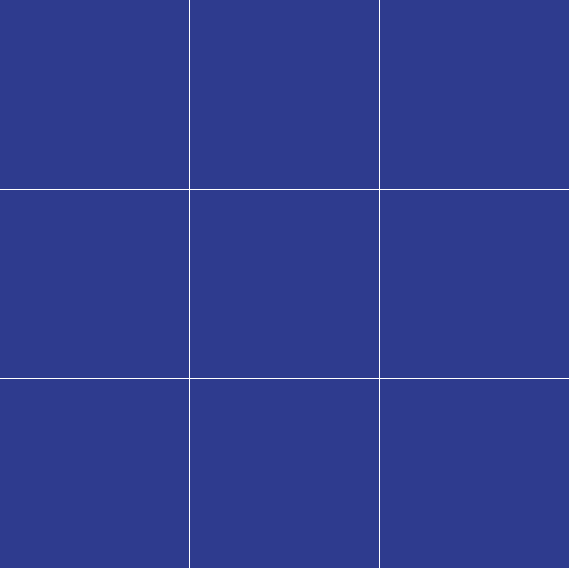
\includegraphics[width=0.3\textwidth]{11_basics/grid00.png}
  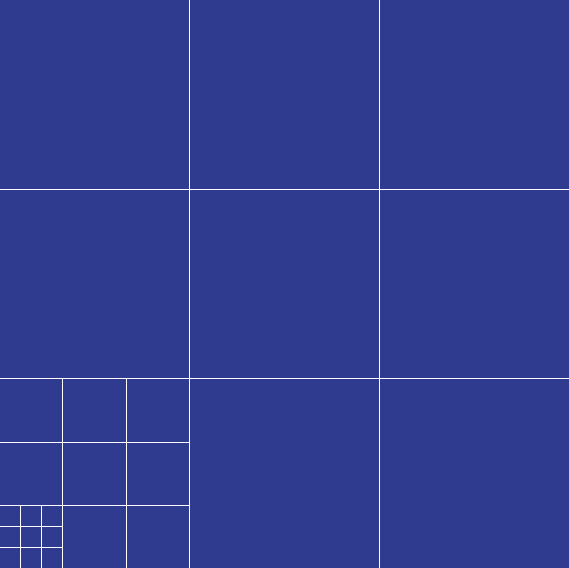
\includegraphics[width=0.3\textwidth]{11_basics/grid01.png}
  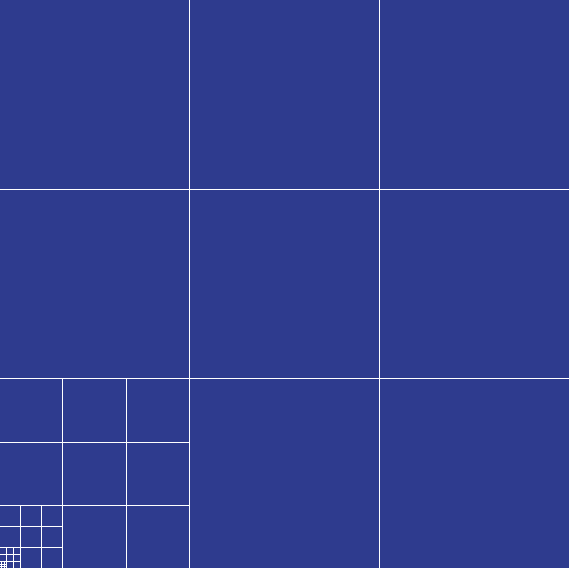
\includegraphics[width=0.3\textwidth]{11_basics/grid02.png}
\end{center}


\section{What happens}


\begin{center}
  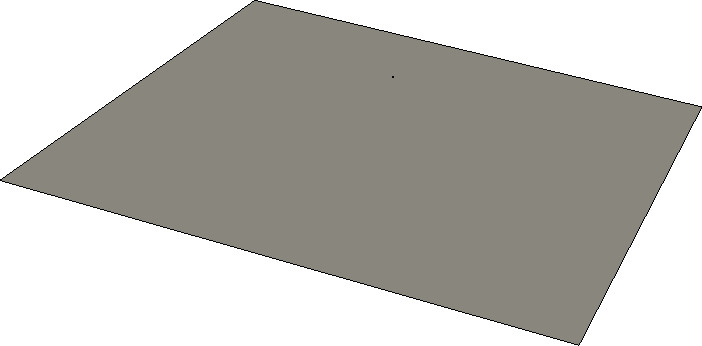
\includegraphics[width=0.45\textwidth]{11_basics/construction00.png}
  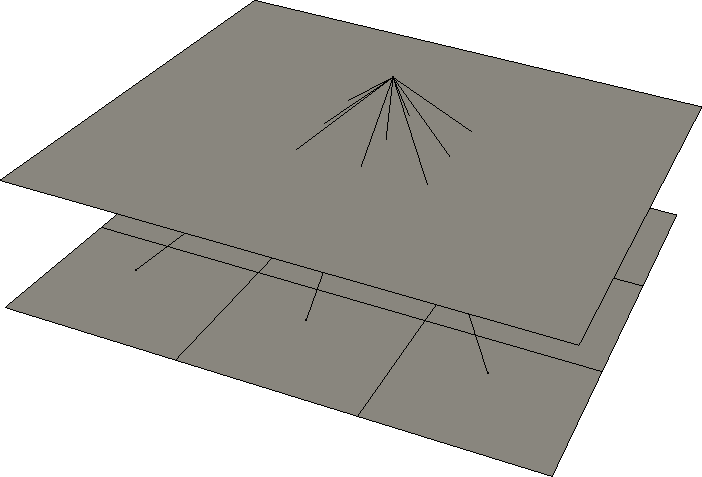
\includegraphics[width=0.45\textwidth]{11_basics/construction01.png}
  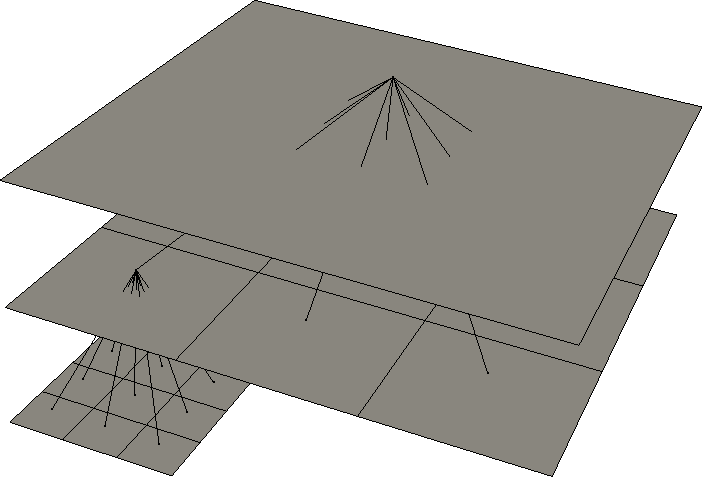
\includegraphics[width=0.45\textwidth]{11_basics/construction02.png}
  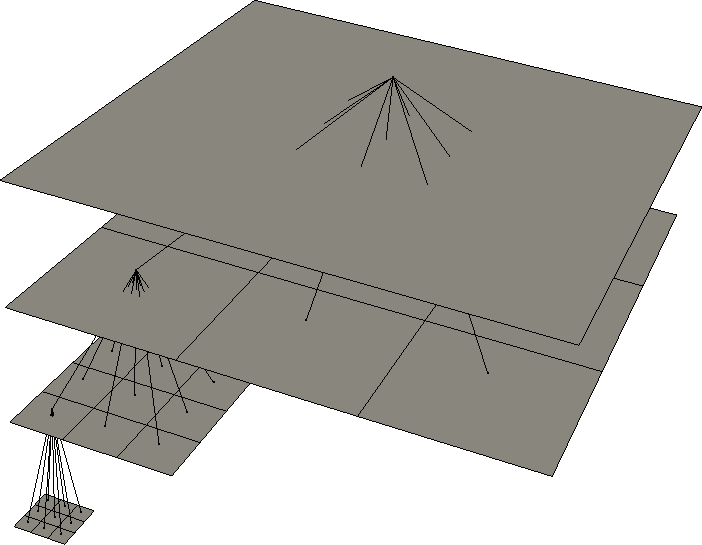
\includegraphics[width=0.45\textwidth]{11_basics/construction03.png}
\end{center}

% UserInterface interpretieren
% Welche events sind da
% was passiert
% Log lesen
% 
% 



\section{Data model}
Prior to a discussion of Peano's data model, it might make sense to load all the
files \texttt{grid-level-?-0.vtk} into your favourite visualisation software.
Dilate them according to their level encoded in the name.
In Paraview, you have to select each file, apply
Filters/Alphabetical/Transform, and dilate each file by -0.2 along the z-axis
per level.
You might end up with something alike:



\begin{center}
  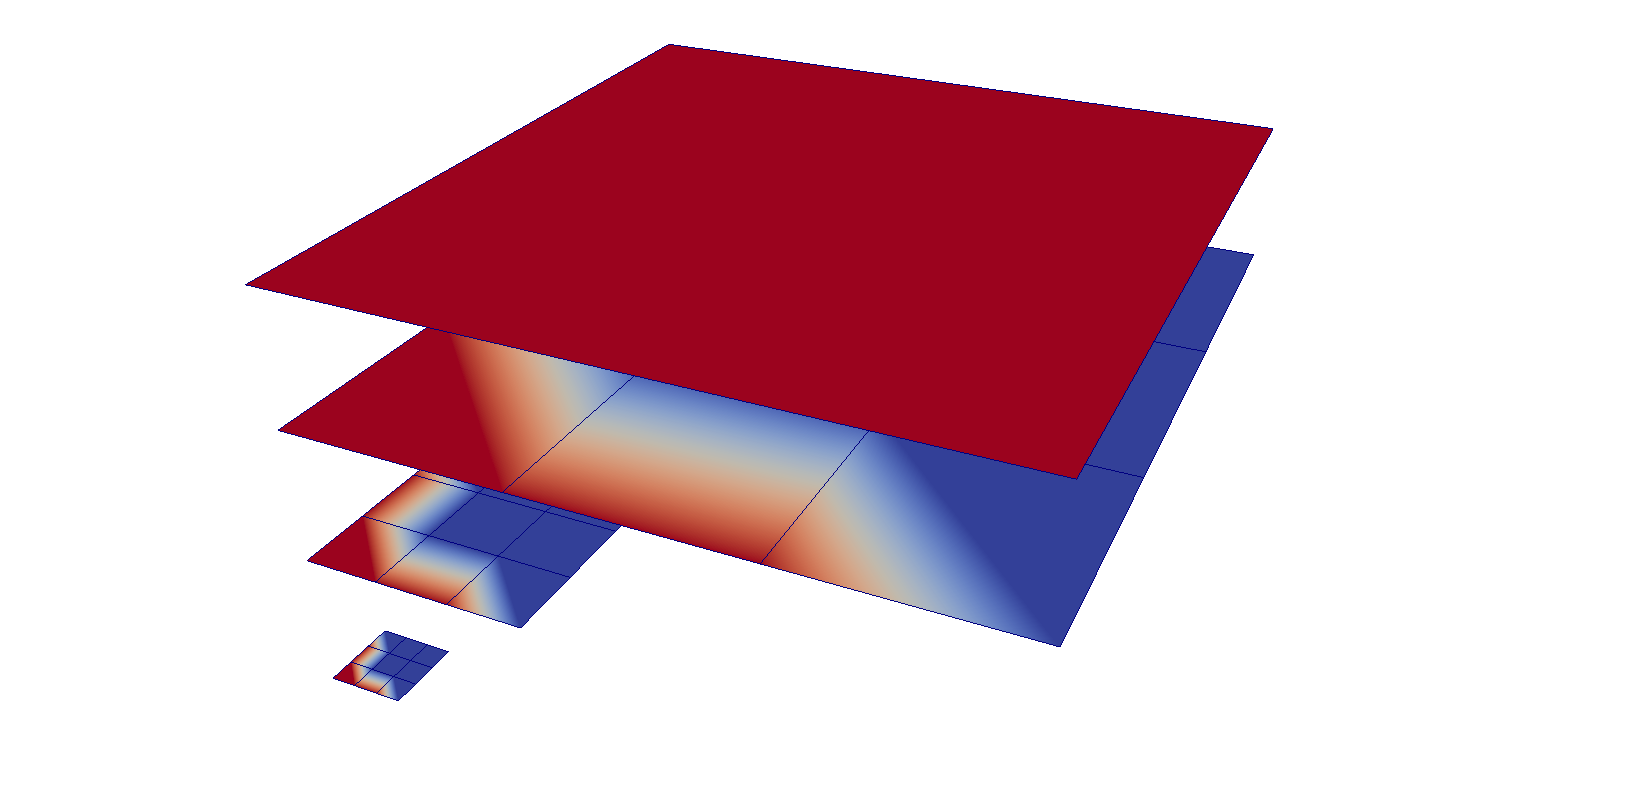
\includegraphics[width=0.8\textwidth]{11_basics/tree00.png}
\end{center}

\noindent
Again, feel free to create a video that shows how additional levels are added in
each step.
There's a more elegant way to end up with a similar picture. 
I once created a graph visualiser that is today also available as predefined
mapping. Just modify your adapters as follows:

\begin{code}
adapter:
  name: CreateGridAndPlot
  merge-with-user-defined-mapping: CreateGrid
  merge-with-predefined-mapping: VTK2dTreeVisualiser(tree,getLevel)
\end{code}

\noindent
This time, creating a video should be straightforward.
\begin{center}
  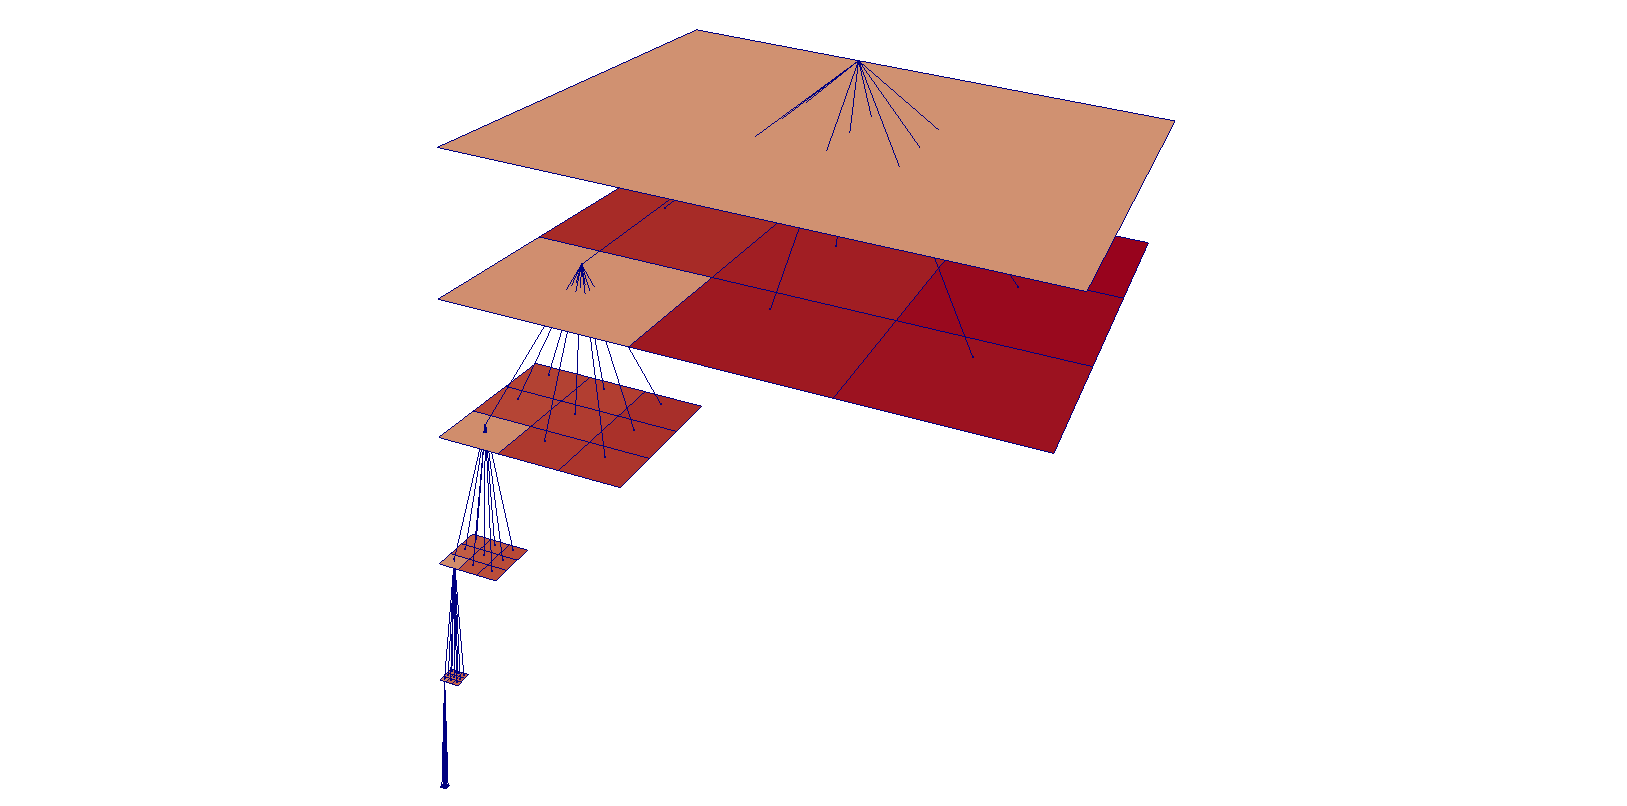
\includegraphics[width=0.8\textwidth]{11_basics/tree01.png}
\end{center}

% Data Model
% Visualisierung von Einbettung
% Wo liegen welche Daten
% 
% Remark: How to realise degrees of freedom associated to faces or edges
% 


\section{Counting vertices}
% We could use the repository's operations
% Do it yourself and then compare
% Finale: Vertices zaehlen
% Den Wert von einem double umsetzen


